% ======================================================================
% chain_unified.tex  (2026-11-09)
%
% One document for the whole analysis chain, from a pixel's count to arsenic
% mass.  It replaces, as the working description, these drafts (left
% unchanged as the record):
%   analysis_chain.tex (10-03), chain_derivation1.tex (10-05),
%   chain_derivation2.tex (10-22), chain_derivation.tex (10-23),
%   chain_derivation_B.tex (10-27; Bill's lines 1-171 set the notation),
%   docs/pad_light_physics_2026-10-25.md,
%   docs/color_coordinates_brightness_2026-10-25.md,
%   docs/edge_profile_plan_2026-10-23.md.
% Appendix A maps every earlier symbol to this document's.
% Worked-example numbers were checked by a throwaway script (session
% scratchpad, ex.py), not by hand only.
% ======================================================================
\documentclass[11pt,letter]{article}

\usepackage[margin=2.5cm]{geometry}
\usepackage{amsmath}
\usepackage{amssymb}
\usepackage{bm}
\usepackage{booktabs}
\usepackage{longtable}
\usepackage{array}
\usepackage{ragged2e}
\usepackage{seqsplit}
\usepackage{enumitem}
\usepackage[hidelinks]{hyperref}
\usepackage{cleveref}
\usepackage{setspace}
\usepackage{graphicx}
\graphicspath{{figs/}}
\setstretch{1.15}
\setlength{\emergencystretch}{3em}
\newcolumntype{L}[1]{>{\RaggedRight\arraybackslash}p{#1}}

%----------------------------------------------------------------------
%  Text helpers
%----------------------------------------------------------------------
\newcommand{\file}[1]{\texttt{\seqsplit{#1}}}
\newcommand{\COMMENT}[1]{}
\newcommand{\open}[1]{\textbf{[Open item~\ref{#1}]}}
\newcommand{\Lten}{\log_{10}}
\newcommand{\one}{\mathbf{1}}
\newcommand{\vy}{\mathbf{y}}
\newcommand{\vb}{\mathbf{b}}
\newcommand{\vA}{\mathbf{A}}
\newcommand{\mS}{\mathbf{S}}
\newcommand{\mM}{\mathbf{M}}
\newcommand{\vm}{\mathbf{m}}
\newcommand{\va}{\mathbf{a}}
\newcommand{\Rinf}{R_{\infty}}

% Step numbers for the step sections, so cross-references read "step 3 (§6)".
\makeatletter
\newcommand{\defstep}[2]{\@namedef{stepno@#1}{#2}}
\newcommand{\sno}[1]{step~\@nameuse{stepno@#1}}
\newcommand{\Sno}[1]{Step~\@nameuse{stepno@#1}}
\makeatother
\newcommand{\sref}[1]{\sno{#1} (\S\ref{#1})}
\newcommand{\Sref}[1]{\Sno{#1} (\S\ref{#1})}
\newcommand{\psref}[1]{\sno{#1}, \S\ref{#1}}  % inside parentheses
\defstep{sec:phi}{3}
\defstep{sec:lineup}{4}
\defstep{sec:white}{5}
\defstep{sec:ratio}{6}
\defstep{sec:absorbance}{7}
\defstep{sec:color}{8}
\defstep{sec:mass}{9}

\newenvironment{evidence}{\par\medskip\noindent\textbf{Evidence still
needed.}\begin{itemize}[nosep]}{\end{itemize}\medskip}

\title{The analysis chain, from a pixel's count to arsenic mass\\
\large One unified derivation}
\author{Colorimeter project --- pad analysis}
\date{Draft for Bill's review, 2026-11-09.  No code is changed by this
document.}

\begin{document}
\maketitle

\begin{abstract}
\noindent
The chain turns two photos of the same indicator pad, one before and one
after exposure to arsine, into an arsenic mass.  Almost all of it rests on one
fact, proved in \sref{sec:ratio}: dividing a pad pixel in the post-image by
the same piece of pad in the pre-image, and correcting for the change in
lighting with the gray chips, leaves only the change that the dye made.  The
other steps handle what that division cannot: noise in the pre-image
(\psref{sec:white}), the conversion to a scale where dyes add
(\psref{sec:absorbance}), the split into yellow and brown (\psref{sec:color}),
and the conversion to mass (\psref{sec:mass}).  Each step states its
assumptions, proves its result in a few lines, and gives a small worked
example.  What is not yet established is listed as numbered open items in
\cref{sec:open}.
\end{abstract}

\tableofcontents

%======================================================================
\section{What the chain does, and how big things are}
\label{sec:scope}

The instrument photographs a paper indicator pad on a plastic strip, under
one LED color at a time, with a gray reference chip on each side of the strip
in the same photo.  It does this twice: the \textbf{pre-image}, of the dry
pad before exposure to arsine, and the \textbf{post-image}, after.  Arsine
reacts with the mercuric bromide in the paper and leaves a yellow-to-brown
stain.  The chain measures that stain, pixel by pixel, and turns it into
the mass of arsenic that made it.

\textbf{The scale of things} (as of 2026-11; sources in \cref{app:sources}).
Every step below is compared with these numbers, so that no step is
polished beyond what can matter.  A is absorbance (\psref{sec:absorbance}):
bigger means darker; 0.001\,A is about 0.23\,\% of the light.

\medskip
\begin{tabular}{@{}L{7.5cm}L{7.0cm}@{}}
\toprule
Source of spread & Rough size \\
\midrule
Camera noise, one pixel, one photo & about 0.002\,A \\
Paper texture, pixel to pixel & 0.006--0.008\,A (1.4--1.8\,\%) \\
Darkening at the pad's edge & up to 30\,\% in the outermost layer
  pixel, 2--3 pixels wide \\
Gray-polynomial curvature between the chips & 2--4\,\% in absolute
  reflectance (cancels in the ratio, \psref{sec:phi}) \\
Replicate strips at the same concentration & disagree by about a factor of
  1.9 \\
\bottomrule
\end{tabular}

\medskip
\noindent The last row is far larger than all the others.  The chain's job
is to add as little as possible to it, simply and provably, not to remove
every effect of 1\,\%.

\textbf{Pixels.}  ``Pixel'' means a pixel of one Bayer layer, 0.12\,mm on
the pad.  The pad is about $42 \times 54$ such pixels.  A
\textbf{channel} is one LED color seen through one Bayer layer, for example
\texttt{cyan.B}.  The six channels the analysis uses are \texttt{violet.B},
\texttt{royal\_blue.B}, \texttt{cyan.B}, \texttt{green.Gb}, \texttt{green.Gr}
and \texttt{photo\_red.R}.  The two green layers are never averaged
together: they differ by 1.5\,\% under some LEDs.  Steps 0--7
(through \S\ref{sec:absorbance}) are done for each channel on its own.

%======================================================================
\section{Words and symbols}
\label{sec:symbols}

\subsection{Conventions}

\begin{itemize}[nosep]
  \item A \textbf{prime} ($'$) marks the pre-image: $n'_p$ is the pre-image
    count, $n_p$ the post-image count.
  \item The subscript $p$ names one pixel.  Rows and columns, $(i, j)$, are
    used only for the edge bands.
  \item \textbf{Reflectance quantities} use the Latin letters $r$, $s$,
    $d$, $D$, $R$: bigger means \emph{lighter}.  \textbf{Absorbance
    quantities} use $A$ and $a$: bigger means \emph{darker}.
  \item Bold lowercase ($\vy$) is a list of numbers, one per channel.  Bold
    uppercase ($\mS$) is a table of numbers (a matrix).
  \item Each symbol has one meaning in this whole document.
\end{itemize}

\subsection{The symbols}

\begin{longtable}{@{}L{2.3cm}L{10.6cm}L{1.6cm}@{}}
\toprule
Symbol & Meaning & First in \\
\midrule
$I_p$ & light falling on the spot of pad seen by pixel $p$ & \S\ref{sec:light} \\
$s$ & specular fraction: the share of $I$ that bounces off the top surface
  like a mirror & \S\ref{sec:light} \\
$\alpha,\ \varepsilon,\ \tau$ & of the light that enters the paper, the
  fractions absorbed, lost out the cut edge, and lost out the back
  & \S\ref{sec:light} \\
$d$ & diffuse reflectance: the share of $I$ that comes back out of the top
  after wandering in the paper & \S\ref{sec:light} \\
$r = s + d$ & total reflectance & \S\ref{sec:light} \\
$\kappa$ & the share of the light leaving the top that the camera collects,
  times the camera's counts per unit of light & \S\ref{sec:light} \\
$n_p$ & a pixel's count, dark level removed, in DN (digital numbers) &
  \S\ref{sec:light} \\
$e$ & the dark level: the dark frame's whole-frame average & \S\ref{sec:light} \\
$D_p$ & bulk diffuse reflectance: what $d$ would be at $p$ far from any
  edge, with average texture.  Set by the paper and its dye & \S\ref{sec:factors} \\
$\ell_p$ & edge factor: the share of light kept at pixel $p$ because it is
  near a cut edge; 1 far from the edges & \S\ref{sec:factors} \\
$f_p$ & fiber factor: the pixel's own texture, average 1 & \S\ref{sec:factors} \\
$P_p$, $c$, $c'$ & shape of the light over the stage (mean 1), and its
  level in the post-image and in the pre-image & \sno{sec:phi} \\
$g_1,\ g_2$ & mean count over gray chip 1 and gray chip 2 & \sno{sec:phi} \\
$\rho_g$, $\kappa_g$ & the gray chips' reflectance; the camera's share for
  the chips & \sno{sec:phi} \\
$\Phi$ & the gray-chip ratio $g/g'$: how much more light the post-image
  got & \sno{sec:phi} \\
$w_1,\ w_2$ & the gray polynomial's weights on the two chips & \sno{sec:phi} \\
$W_p$, $h_q$ & the pre-image lined up on the post-image's pixels; the
  lining-up weights & \sno{sec:lineup} \\
$S'$, $\widetilde W_p$ & smooth part of the pre-image; the model white
  $S'\ell_p$ & \sno{sec:white} \\
$\widehat W_p$, $\lambda$ & the white used in the ratio, a blend of $W_p$
  and $\widetilde W_p$; the weight on $W_p$ & \sno{sec:white} \\
$\delta_p,\ \delta'_p$ & camera noise in the post-image and in the
  pre-image, as fractions & \sno{sec:white} \\
$\eta_p$ & the texture that the model white leaves out, as a fraction &
  \sno{sec:white} \\
$\Rinf$ & the post-image divided by the white: 1 for unreacted pad,
  smaller where dye is & \sno{sec:ratio} \\
$A$ & absorbance, $A = -\Lten \Rinf$: 0 for unreacted pad, bigger is darker
  & \sno{sec:absorbance} \\
$\vA_p$ & the pixel's absorbances in all channels, one number per channel &
  \sno{sec:color} \\
$\one,\ \vy,\ \vb$ & the brightness direction (all ones); the yellow and
  the brown absorbance lists, per unit amount & \sno{sec:color} \\
$\gamma_p,\ c_{Y,p},\ c_{B,p}$ & the pixel's brightness shift, yellow
  amount, brown amount & \sno{sec:color} \\
$\mS,\ \mM$ & the table $[\one\ \vy\ \vb]$; the measuring table that reads
  amounts from $\vA$ & \sno{sec:color} \\
$N_1, N_2, N_3$ & numbers of arsenic atoms at a pixel holding 1, 2 or 3
  mercury bromide groups & \sno{sec:mass} \\
$\va_1, \va_2, \va_3$ & absorbance per atom of each kind, one number per
  channel & \sno{sec:mass} \\
$F$ & the curve that turns a pixel's yellow and brown amounts into mass,
  found by calibration & \sno{sec:mass} \\
$m_p,\ m_\Sigma$ & arsenic mass at pixel $p$; total over the pad &
  \sno{sec:mass} \\
\bottomrule
\end{longtable}

\subsection{Words}

\begin{tabular}{@{}L{3.2cm}L{11.6cm}@{}}
\toprule
Word & Meaning in this document \\
\midrule
pre-image, post-image & photos of the strip before and after exposure to
  arsine \\
exposure\_us & the camera's exposure time, in microseconds.  ``Exposure'' alone
  means exposure to arsine \\
gray chip & a gray reference square fixed to the stage, one on each side
  of the strip.  Not a ``patch'', which is a color on the calibration card \\
pad & the paper indicator on the strip \\
texture & the paper's own fixed pixel-to-pixel pattern.  It moves with the
  strip.  It is not noise \\
noise & random change from one photo to the next at the same pixel \\
white & the pre-image's value for a pixel, lined up and scaled, used as
  the divisor \\
\bottomrule
\end{tabular}

%======================================================================
\section{Light at one pixel}
\label{sec:light}

\subsection{Where the light goes}

Light $I$ falls on the small spot of pad that pixel $p$ sees.  (Drop the
$p$ for now.)  A small share $s$ bounces off the top surface like a mirror,
about 4\,\% for paper.  The rest, $(1 - s)\,I$, enters the paper.  Inside,
each photon wanders from fiber to fiber until it ends in exactly one of four
places: absorbed (by the paper or the dye), lost out a cut edge, lost out
the back, or back out of the top.  Light is not created or destroyed, so the
four parts add up to what entered:
\begin{equation}
  (1 - s)\, I = P_\text{abs} + P_\text{edge} + P_\text{back} + P_\text{top} .
  \label{eq:balance}
\end{equation}
Divide by $(1 - s)\,I$ and name the shares of the light that entered:
\begin{equation}
  \alpha = \frac{P_\text{abs}}{(1-s)I}, \qquad
  \varepsilon = \frac{P_\text{edge}}{(1-s)I}, \qquad
  \tau = \frac{P_\text{back}}{(1-s)I} .
\end{equation}
Then \eqref{eq:balance} gives the light leaving the top,
\begin{equation}
  P_\text{top} = (1 - s)\, I\, (1 - \alpha - \varepsilon - \tau) .
\end{equation}
The \textbf{diffuse reflectance} is that light as a share of $I$, and the
\textbf{total reflectance} adds the mirror bounce:
\begin{equation}
  d = \frac{P_\text{top}}{I} = (1 - s)(1 - \alpha - \varepsilon - \tau),
  \qquad r = s + d .
  \label{eq:d}
\end{equation}
(Earlier drafts wrote ``$I d$ is the light that enters the paper''.  The light
that enters is $(1-s)\,I$; $d$ is what comes back out.)

\subsection{What the camera counts}

The camera collects a fixed share of the light leaving the top and turns it
into counts; $\kappa$ is that share times the counts per unit of light.
After the dark level is removed (step~0 below), the count is
\begin{equation}
  n = \kappa\, I\, d .
  \label{eq:count}
\end{equation}
\textbf{A count is not a reflectance.}  $n$ carries the light level $I$ and
the camera's $\kappa$.  It becomes a reflectance only after dividing by
something that carries the same $I$ and $\kappa$: a gray chip, or the same
pad in another photo.

\subsection{Why the mirror bounce is left out}
\label{sec:specular}

The LEDs are 20--28$^\circ$ from straight down, and the camera looks straight
down.  A mirror bounce leaves at the same angle on the other side, so it
misses the lens.  That is why \eqref{eq:count} has $d$ and not $r$.  The share
$s$ still matters as the factor $(1 - s)$ on the light that enters.  That
factor is the same in both photos, so it cancels in \sref{sec:ratio}.

\textbf{Why this needs the geometry, not just ``$s$ is small''.}  Suppose a
share of the mirror bounce did reach the camera.  It would be \emph{added}
to the count: $n = \kappa I d + \kappa_s I s$.  An added term does not
cancel in a ratio.  Example: paper $d' = 0.8$, dyed $d = 0.4$, so the true
ratio is 0.5.  With an added $\kappa_s s/\kappa = 0.02$, the measured ratio is
$(0.4 + 0.02)/(0.8 + 0.02) = 0.512$: the dye reads 0.011\,A too light.  So
the assumption is that no mirror bounce reaches the lens \open{op:specular}.

\subsection{Step 0: the dark level and hot pixels (settled)}

The camera reads a little with no light.  Light adds to it, so it is removed
by subtraction, before any division: $n = n_\text{raw} - e$, where $e$ is
the whole-frame average of the dark frame, one number per Bayer layer per
photo.  Pixels whose dark level is reliably high (hot pixels) are masked
out.  This is settled and described in
\file{tex/dark\_signal\_characterization.tex}; it is not repeated here.

\subsection{Light adds, so averages are done on light}
\label{sec:lightadds}

A pixel records the light over its area.  Any step that stands for ``the
light over a shifted or a larger area'' (lining up, smoothing, a band mean)
must therefore be an ordinary average of counts or of reflectance, never of
absorbance.  Example: half a pixel returns 1.0 of the white, the other half
0.5.  The pixel records $0.75$, which is $A = 0.125$.  Averaging the two
halves' absorbances, $0$ and $0.301$, gives $0.151$: wrong.

%======================================================================
\section{From a sum of losses to a product of factors}
\label{sec:factors}

The ratio in \sref{sec:ratio} cancels things that \emph{multiply} the light.
The bracket $(1 - \alpha - \varepsilon - \tau)$ is a \emph{sum} of losses.  So
the chain needs one assumption that turns it into a product.

\textbf{Assumption F (factor form).}  At pixel $p$, the diffuse reflectance
is
\begin{equation}
  d_p = (1 - s)\; f_p\; \ell_p\; D_p ,
  \label{eq:factor}
\end{equation}
where
\begin{itemize}[nosep]
  \item $D_p$ is the bulk diffuse reflectance: what $d$ would be here far
    from any edge, with average texture.  It holds the absorption $\alpha$
    and the back loss $\tau$.  \textbf{The dye changes only $D_p$.}
  \item $\ell_p$ is the edge factor.  It holds the edge loss $\varepsilon$:
    $\ell_p = 1$ far from the edges and less than 1 near them.
  \item $f_p$ is the fiber factor: the pixel's own texture (local fiber
    density, fiber direction, the surface's tilt), average 1.
\end{itemize}
$s$, $\ell_p$ and $f_p$ are the same in both photos.

\textbf{Why it is only approximately true.}  The four shares in
\eqref{eq:balance} compete for the same photons: a photon that is absorbed
cannot also leave by the edge.  Dye raises $\alpha$, which shortens the
photons' paths, so it lowers $\varepsilon$ and $\tau$.  Assumption~F ignores
this.  Two known places where it shows:
\begin{itemize}[nosep]
  \item \textbf{Dye at the edge.}  With dye, fewer photons reach the edge,
    so $\ell_p$ moves toward 1.  Dividing by the pre-image's $\ell_p$ then
    removes too much, and a dyed edge reads lighter than it is
    \open{op:dyededge}.
  \item \textbf{Texture inside the dye.}  In the red channel, the pre-image's
    fine texture carries into the post-image with a slope of about 0.3
    inside the dot, against 0.43--0.82 on the white pad around it (16 of 18
    pads; test~B, \file{docs/resume\_prompt\_pad\_light\_physics.md}).  So
    inside the dye $f_p$ is weaker than in the pre-image \open{op:texture}.
\end{itemize}

\textbf{What makes $\ell$ and $f$} (a working picture, not a finding).
\begin{itemize}[nosep]
  \item Edge: light spreads sideways in paper over a length $L$ and is lost
    out the cut edge.  For an unlit edge this gives
    $\ell(x) = 1 - \tfrac12 e^{-x/L}$ at distance $x$ from the edge.  It
    fits the left edge of C1032 \texttt{royal\_blue.B} with
    $L = 0.10$\,mm, inside the published range for paper, but it is one
    pad and one channel.  Light entering the lit edge faces works the other
    way and is not modeled
    (\file{docs/pad\_light\_physics\_2026-10-25.md}, \S4.2 and \S4.8).
  \item Texture: its cause is not settled.  A shadow cast by fibers is
    unlikely: a one-pixel shadow needs bumps 0.23\,mm or more tall, as tall
    as the pad.  The candidates are the paper's local properties, thickness
    over the slightly see-through backing, and surface tilt (same note,
    \S5--6).  The chain does not depend on which: it only needs $f_p$ to be
    fixed to the paper and the same in both photos.
\end{itemize}

Putting \eqref{eq:factor} into \eqref{eq:count}, the two counts at pixel
$p$ are
\begin{equation}
  n_p = \kappa (1 - s)\, I_p\, f_p\, \ell_p\, D_p , \qquad
  n'_p = \kappa (1 - s)\, I'_p\, f_p\, \ell_p\, D'_p .
  \label{eq:counts}
\end{equation}
The second assumes the same piece of paper is at pixel $p$ in both photos;
\sref{sec:lineup} makes that true.

%======================================================================
\section{Steps 1 and 2: the pre-image and the post-image}
\label{sec:photos}

\textbf{Step 1} photographs the dry pad, the \textbf{pre-image}, in every
channel, with both gray chips in the same photo.  (The current pre-images
hold five LEDs, \texttt{violet}, \texttt{royal\_blue}, \texttt{cyan},
\texttt{green} and \texttt{photo\_red}, on all their usable Bayer layers;
checked on C1017, C1025, C1032, C1036 and C1038.)  \textbf{Step 2}
photographs the same strip after exposure, the \textbf{post-image}, the same
way.  Both are dark-corrected (step~0).  For each photo and channel the
chain keeps:
\begin{itemize}[nosep]
  \item the pad pixels' counts, $n'_p$ and $n_p$;
  \item the mean count over each gray chip, $g'_1, g'_2$ and $g_1, g_2$.
\end{itemize}
The two photos may use different exposure\_us, and the LEDs may drift
between them.  The light levels $I'_p$ and $I_p$ are therefore different,
and unknown.  The strip is taken out and put back between the photos, so it
sits a fraction of a pixel to a few pixels differently.

%======================================================================
\section{Step 3: the gray-chip ratio, and why the gray polynomial can wait}
\label{sec:phi}

\subsection{The ratio}

\textbf{Assumption G (same shape of light).}  The light over the stage has
the same \emph{shape} in both photos and differs only in level:
\begin{equation}
  I_p = c\, P_p, \qquad I'_p = c'\, P_p ,
  \label{eq:shape}
\end{equation}
where $P_p$ is the shape, fixed by where the LEDs are, and $c$, $c'$ are
the levels (exposure\_us times LED output).

A gray chip has reflectance $\rho_g$ that never changes, and no texture or
edge in its mean.  Its mean count is $\kappa_g\, I\, \rho_g$, so for chip 1
\begin{equation}
  \frac{g_1}{g'_1} = \frac{\kappa_g\, c\, \bar P_1\, \rho_g}
                          {\kappa_g\, c'\, \bar P_1\, \rho_g}
                   = \frac{c}{c'} ,
\end{equation}
where $\bar P_1$ is the mean shape over chip 1.  Chip 2 gives the same
$c/c'$.  Call it
\begin{equation}
  \Phi = \frac{c}{c'} = \frac{g_1}{g'_1} = \frac{g_2}{g'_2} .
  \label{eq:phi}
\end{equation}
By \eqref{eq:shape}, $I_p / I'_p = c\,P_p / (c'\,P_p) = \Phi$ at
\emph{every} pixel, chips and pad alike: the shape $P_p$ cancels.  In
practice $\Phi$ is taken as the mean of $g_1/g'_1$ and $g_2/g'_2$.

This is Bill's ``scale the pre-image to the post-image with the ratio of
the gray chips'': the pre-image multiplied by $\Phi$ is what the pre-image
would have read under the post-image's light.

\subsection{The gray polynomial cannot change the ratio by more than the
chips disagree}

At run time the gray polynomial reduces to two weights per pad pixel: the
gray level it predicts at pixel $p$ is $G_p = w_1 g_1 + w_2 g_2$, and
$G'_p = w_1 g'_1 + w_2 g'_2$ in the pre-image, with the same weights
(memory \file{project\_flatfield\_anchor}).  The weights are positive,
because the pad lies between the chips.  Write $\Phi_1 = g_1/g'_1$ and
$\Phi_2 = g_2/g'_2$.  Then the ratio the polynomial would use is
\begin{equation}
  \frac{G_p}{G'_p}
  = \frac{w_1 \Phi_1 g'_1 + w_2 \Phi_2 g'_2}{w_1 g'_1 + w_2 g'_2}
  = u\,\Phi_1 + (1 - u)\,\Phi_2, \qquad
  u = \frac{w_1 g'_1}{w_1 g'_1 + w_2 g'_2} .
  \label{eq:polyratio}
\end{equation}
Since $0 < u < 1$, this is a weighted average of $\Phi_1$ and $\Phi_2$.  So:
\begin{itemize}[nosep]
  \item If the chips agree, $\Phi_1 = \Phi_2 = \Phi$, then
    $G_p/G'_p = \Phi$ exactly, whatever the polynomial is.  The polynomial
    is immaterial to the ratio.
  \item If they disagree, the polynomial's ratio still lies between
    $\Phi_1$ and $\Phi_2$, so using their plain mean is off by at most half
    the gap, $|\Phi_1 - \Phi_2|/2$.  As a share of $\Phi$ and in absorbance,
    the most this can be is $0.434 \times |\Phi_1 - \Phi_2| / (2\Phi)$.
\end{itemize}
The polynomial is still needed for \emph{absolute} reflectance (a pad's
reflectance compared with the chip's), where its 2--4\,\% curvature
matters.  The ratio chain does not use absolute reflectance.  Whether the
chips agree is one number per sample and channel.  Tabulating it is
deferred (Bill, 2026-11-09) \open{op:phi}.

\textbf{Example.}  Chips $\rho_g = 0.45$, post-image level $c = 1000$,
pre-image $c' = 600$, $P = 1$ at both chips: $g = 450$, $g' = 270$,
$\Phi = 1.667$ from either chip.

\begin{evidence}
  \item A table of $\Phi_1/\Phi_2 - 1$ over all samples and channels, and
    the largest error it implies in A.
\end{evidence}

%======================================================================
\section{Step 4: line up the pre-image}
\label{sec:lineup}

\textbf{In words.}  The strip was put back between the photos, so the same
piece of pad sits at slightly different pixels.  Lining up moves the
pre-image onto the post-image's pixels, so that each post-image pixel is
paired with the same piece of paper.  Without it, $f_p$ and $\ell_p$ do not
cancel.  An unnoticed shift of 0.2\,pixel leaves a false change of up to
0.03\,A in the outermost pixel at the edge
(\file{docs/edge\_profile\_plan\_2026-10-23.md}, \S3).

\textbf{Method.}  The shift comes from the pad's fitted edges in each photo
(\file{analysis\_1.pre\_to\_post}).  The piece of paper at post-image pixel
$p$ sat, in the pre-image, between pixels.  Its value is a weighted average
of the nearest pre-image pixels $q$, with weights $h_q$ set by how close
each one is:
\begin{equation}
  W_p = \sum_q h_q\, n'_q , \qquad \sum_q h_q = 1 ,\ h_q \ge 0 .
  \label{eq:W}
\end{equation}
This is an average of light, as \cref{sec:lightadds} requires.

\textbf{Result.}  With the paper put back in place (Assumption~L: lining up
places the same paper on the same pixel, to a small fraction of a pixel),
\begin{equation}
  W_p = \kappa (1 - s)\, I'_p\, f_p\, \ell_p\, D'_p ,
  \label{eq:Wresult}
\end{equation}
which is \eqref{eq:counts} for the pre-image, now on the post-image's
pixels.  The averaging in \eqref{eq:W} also blurs the texture slightly;
that is one reason the texture does not carry over perfectly, and it is
counted with the texture in \sref{sec:white}.

\subsection{How well lining up works (proof-of-concept study, 2026-11-11)}
\label{sec:lineupcheck}

\textbf{Question.}  Does lining up by the fitted edges put the same paper on
the same pixel in holders F, G and H, and how much does what is left over
matter at the edge?  Stop when the false change is under 0.002\,A beyond the
outermost band (work plan, step~1).

\textbf{The measuring stick: the paper's texture.}  The paper has its own
fixed pixel-to-pixel pattern, which moves with the strip.  Take
$\Lten R$ in photo\_red.R (which the yellow dye barely absorbs) and subtract
its 2-pixel smooth; what is left is the texture.  If the post-image's
texture matches the lined-up pre-image's best after an extra shift
$(\Delta y, \Delta x)$, the edge fits were off by that much.  This measure
does not depend on any edge fit.

\textbf{Each photo's own error.}  The strip is reseated between repeats, so
every pre-image of a sample can be paired with every post-image (124 pairs
over C1038--C1045).  For pre-image $i$ and post-image $j$ the leftover shift
is modeled as $r_{ij} = a_j - b_i$ plus measurement noise, where $a_j$ and
$b_i$ are each photo's own edge-fit error (fitted position minus the
position the texture says).  Least squares gives $a$ and $b$, with the mean of
$b$ set to zero, since only differences are seen.

\textbf{What was found, and fixed.}  The post-image sides were fitted
0.5--0.8\,px too wide in C1041 and C1044, and two G1 post-images
(C1045rep3, rep4) could not be fitted at all.  Two causes:
\begin{itemize}
  \item padrect put each side where the brightness crosses half the pad's
    level.  Where dye darkens the paper next to the edge, that crossing
    slides outward.
  \item padrect guessed the holder from the last rows of the crop, which in
    holder G1 are the window's lower edge, so the guess could go either way.
\end{itemize}
The fix (Bill, 2026-11-11), now in \file{padrect.py} and
\file{analysis\_1.pad\_of}: for the cassette holders the layout comes from
the sample's \texttt{cap\_style}, and each side is placed where the
brightness falls most steeply to the dark frame, looked for only within
2\,px of a guide.  A post-image is guided by its own file's pre-image (the
measured movement between them is at most 1.23\,px); a pre-image is guided
by its own first fit.  The half-level rule stays for older holders; the
last commit before the change is 50b70a9.

\textbf{Result, with the guided fits} (\cref{fig:step1_edgefit_error}):
\begin{itemize}
  \item Across the pad, every post-image fit is within $\pm 0.1$\,px of the
    texture except C1041rep4, rep5 ($-0.28$, $-0.25$\,px) and C1039rep5
    ($+0.19$\,px); before the fix the worst was $-0.67$\,px.
  \item Down the pad, the post-image fits sit 0.1--0.3\,px too high.  This
    comes from the ends (top and bottom), not the sides; refining the ends
    is deferred (Bill, 2026-11-11).
  \item The left and right halves of the pad shift by the same amount
    (median difference under 0.1\,px): the paper does not stretch.
  \item False change (positive reads darker than it should): under
    0.0003\,A in the interior; in band~1, a median of 0.005--0.008\,A per
    sample.  Band~1 changes by about 0.1\,A per pixel of misalignment, so
    the stop rule would need about 0.02\,px, finer than the texture can
    measure.  Correcting by the texture shift no longer helps
    (0.004--0.010\,A after), so it is not added.
\end{itemize}
\textbf{Conclusion.}  Lining up is good enough away from the edge.  The
false change left in bands 0 and~1 is handled by the edge bands of
\sref{sec:white}, which take each photo's edges from that photo.
Script: \file{desktop/padanalysis/align\_study.py}, steps 1a--1d; tables in
\file{align\_out/}.

\begin{figure}[h!]
    \centering
    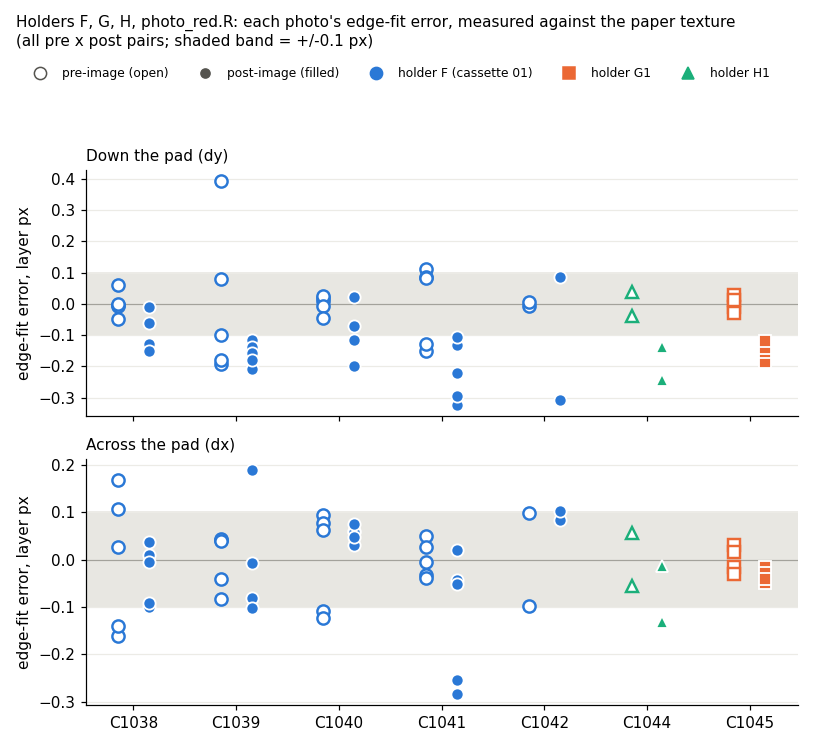
\includegraphics[scale=0.57]{step1_edgefit_error}
    \caption{
    Each photo's edge-fit error, measured against the paper texture, in
    photo\_red.R, with the guided side fits.  Open markers: pre-images;
    filled: post-images.  Top: down the pad; bottom: across the pad.
    Layer pixels, measured from the sample's average pre-image; negative
    means the fit put the pad too high or too far left.  Shaded band
    $\pm 0.1$\,px.  Made by \texttt{align\_study.show\_split}.
    }
\label{fig:step1_edgefit_error}
\end{figure}

%======================================================================
\section{Step 5: the white, one value per pixel}
\label{sec:white}

\subsection{Why the white needs more than the lined-up pre-image}

Without noise, the lined-up pre-image $W_p$ is already the right divisor
(\psref{sec:ratio}).  But each pre-image pixel carries camera noise, and
dividing by it puts that noise into the answer.  Smoothing $W_p$ lowers the
noise but blurs the edge and the texture, which then no longer cancel.
Bill's idea resolves this: model the parts of $W_p$ that are smooth
\emph{along} the edge, average over many pixels to measure them, and keep
the rest of the pixel.

\subsection{The model white: a smooth part and the edge bands}

\textbf{The smooth part.}  Away from the edges, the pre-image is the even
light of the stage on unreacted paper with average texture.  The four LEDs
of a color vary by only 0.09--0.15\,\% over the pad, so this part is
nearly constant.  Call it $S'$; in the symbols of \eqref{eq:Wresult},
$S' = \kappa(1-s)\,I'_p\,D'_p$.  Take it as the mean (or, if a slope
shows, a fitted plane) of $W_p$ over the pad's interior.

\textbf{The edge bands.}  For one edge, group the pad's pixels into bands
one pixel wide by their distance from that edge: band 0 is the outermost,
then band 1, band 2.  Each band runs the length of the edge, leaving out the
corners.  The band's edge factor is its mean over the smooth part:
\begin{equation}
  \ell_k = \frac{\text{mean of } W_p \text{ over band } k}{S'} .
  \label{eq:band}
\end{equation}
Because $f_p$ averages to 1 and the noise averages to 0 over the 40 or so
pixels of a band, $\ell_k$ is nearly free of both.  Pixels past the last
band have $\ell = 1$.  The number of bands is set by the data (decided,
Bill, 2026-11-09): add bands
until a band's mean is within camera noise (0.002\,A) of the interior.  The
measured darkening is 2--3 pixels wide, so expect about three.

\textbf{Corners.}  A pixel near two edges, in band $k$ of one and band $k^*$
of the other, gets the product $\ell_p = \ell_k\, \ell_{k^*}$.  For an evenly
spreading light this is exact at the corner itself and 0.5--1.5\,\% low a
little way in (\file{docs/color\_coordinates\_brightness\_2026-10-25.md},
\S6).

\textbf{The model white} is then $\widetilde W_p = S'\, \ell_p$.  It has the edge and
almost no noise, but not the pixel's own texture.

\subsection{The blend, and the best weight}

\textbf{The white used in the ratio} is a blend of the pixel itself and the
model:
\begin{equation}
  \widehat W_p = \lambda\, W_p + (1 - \lambda)\, \widetilde W_p ,
  \qquad 0 \le \lambda \le 1 .
  \label{eq:blend}
\end{equation}
Both are averages of light, so the blend is too.

\textbf{The errors.}  Let $W^*_p = S' \ell_p f_p$ be the noise-free white.
The measured pixel has noise $\delta'_p$, and the model lacks the texture:
\begin{equation}
  W_p = W^*_p\,(1 + \delta'_p), \qquad
  \widetilde W_p = \frac{W^*_p}{f_p} = W^*_p\,(1 + \eta_p), \quad
  \eta_p = \frac{1}{f_p} - 1 .
  \label{eq:errors}
\end{equation}
$\eta_p$ is the texture the model leaves out: about $-(f_p - 1)$.
Substituting into \eqref{eq:blend},
\begin{equation}
  \widehat W_p = W^*_p\,\bigl[1 + \lambda\,\delta'_p + (1-\lambda)\,\eta_p\bigr] .
  \label{eq:What}
\end{equation}
Steps 6 and 7 (\S\ref{sec:ratio} and \S\ref{sec:absorbance}) show that this bracket goes straight into
the answer, as $0.434 \times [\lambda\,\delta'_p + (1-\lambda)\,\eta_p]$
in absorbance.

\textbf{The best $\lambda$} (Assumption~N: the noise is random, averages
to zero, and is unrelated between the two photos, between pixels, and to
the texture).  Write $\sigma_{\delta'}$ and $\sigma_\eta$ for the spreads
(standard deviations) of $\delta'$ and $\eta$ over the pad.  Spreads of
unrelated quantities add as squares, so the spread the white adds is
\begin{equation}
  s^2(\lambda) = \lambda^2\,\sigma_{\delta'}^2 + (1-\lambda)^2\,\sigma_\eta^2 .
\end{equation}
Its slope in $\lambda$ is $2\lambda\sigma_{\delta'}^2 -
2(1-\lambda)\sigma_\eta^2$.  Setting the slope to zero,
\begin{equation}
  \lambda = \frac{\sigma_\eta^2}{\sigma_{\delta'}^2 + \sigma_\eta^2},
  \qquad
  s^2_\text{min} = \frac{\sigma_{\delta'}^2\,\sigma_\eta^2}
                        {\sigma_{\delta'}^2 + \sigma_\eta^2} .
  \label{eq:lambda}
\end{equation}
It is a minimum, because the curvature
$2(\sigma_{\delta'}^2 + \sigma_\eta^2)$ is positive.  $s^2_\text{min}$ is
$\sigma_{\delta'}^2$ times a number below 1 and $\sigma_\eta^2$ times a
number below 1, so the blend beats both pure choices.  The weight on the
pixel itself is the texture's share of the pre-image's spread: strong
texture calls for the pixel, strong noise calls for the model.  (A longer
form keeps the small noise left in $\widetilde W_p$; it changes the numbers slightly,
not the conclusion.  It is in \file{tex/chain\_derivation\_B.tex},
eq.~\texttt{lambda-exact}.)

\textbf{Example with round numbers.}  Camera noise 0.002\,A is
$\sigma_{\delta'} = 0.0046$; texture 0.007\,A is $\sigma_\eta = 0.016$.  Then
$\lambda = 0.92$.  The white adds 0.0019\,A of spread, against 0.0020\,A
for $\lambda = 1$ (the pixel alone) and 0.0069\,A for $\lambda = 0$ (the
model alone).

\textbf{What the example says.}  With these numbers the texture is larger
than the noise, so the best white is almost the raw pixel, and blending
gains only 0.0001\,A per pixel.  The edge bands matter more for another
reason: they give each photo's edge factor from its own fitted edge, so a
small error in lining up no longer leaves a false change at the edge, and
they are how a change in the edge with dye can be measured
\open{op:dyededge}.  Test~B's slopes (\cref{sec:factors}) say the texture
carries over less than Assumption~F assumes; the best $\lambda$ must be
measured, not taken from these round numbers \open{op:texture}.

\textbf{Noise-free example at an edge pixel.}  $S' = 480$ (pre-image level
600 times paper 0.8), $\ell = 0.70$, $f = 0.98$.  Then $W = 329.28$,
$\widetilde W = 336.0$, and with $\lambda = 0.9$, $\widehat W = 329.95$.  The missing
texture costs $0.434 \times 0.1 \times (1/0.98 - 1) = 0.0009$\,A here, as
\eqref{eq:What} predicts.

\begin{evidence}
  \item Band profiles $\ell_k$ for each edge, several pads and channels,
    raw pre-image beside the model, same color scale.
  \item Measured $\sigma_{\delta'}$ (from repeat photos) and $\sigma_\eta$
    (the texture left after the bands), and the resulting $\lambda$.
  \item Side effect: the blended white must not change the pad's mean.
\end{evidence}

%======================================================================
\section{Step 6: the ratio}
\label{sec:ratio}

\textbf{Definition.}
\begin{equation}
  R_{\infty,p} = \frac{n_p}{\Phi\, \widehat W_p} .
  \label{eq:Rinf}
\end{equation}
In words: the post-image count, divided by what the same piece of paper read
before exposure, scaled to the post-image's light.

\textbf{Without noise} ($\widehat W_p = W_p$).  Substitute \eqref{eq:counts}
for $n_p$, \eqref{eq:Wresult} for $W_p$, and $\Phi = I_p / I'_p$ from
\sref{sec:phi}:
\begin{equation}
  R_{\infty,p}
  = \frac{\kappa (1-s)\, I_p\, f_p\, \ell_p\, D_p}
         {\dfrac{I_p}{I'_p}\;\kappa (1-s)\, I'_p\, f_p\, \ell_p\, D'_p}
  = \frac{D_p}{D'_p} .
  \label{eq:Rinf-clean}
\end{equation}
Everything cancels except the change the dye made to the bulk paper.  It is
1 where there is no dye and smaller where there is.

\medskip
\begin{center}
\begin{tabular}{@{}lll@{}}
\toprule
Factor & What it is & Removed by \\
\midrule
$e$ & dark level & step 0, subtraction \\
$c/c'$, $P_p$ & light level and its shape & step 3, $\Phi$ \\
$\kappa$, $1-s$ & camera, mirror bounce & step 6, the ratio \\
$\ell_p$ & edge & step 6, the ratio (after step 4) \\
$f_p$ & texture & step 6, the ratio (after step 4) \\
$D'_p$ & the unreacted paper & step 6, the ratio \\
\midrule
$D_p/D'_p$ & the dye & \textbf{kept} \\
\bottomrule
\end{tabular}
\end{center}

\textbf{With noise.}  Write the post-image's noise as $n_p = n^*_p(1 +
\delta_p)$.  With \eqref{eq:What},
\begin{equation}
  R_{\infty,p} = \frac{D_p}{D'_p}\;
  \frac{1 + \delta_p}{1 + \lambda\,\delta'_p + (1-\lambda)\,\eta_p} .
  \label{eq:Rinf-noise}
\end{equation}

\textbf{Example} (no noise, $\kappa(1-s) = 1$, $P = 1$, paper $D' = 0.8$,
dyed $D = 0.4$, $\Phi = 1.667$).

\medskip
\begin{center}
\begin{tabular}{@{}lrrrrr@{}}
\toprule
pixel & $f$ & $\ell$ & $n'$ (pre) & $n$ (post) & $\Rinf = n/(\Phi n')$ \\
\midrule
interior & 1.02 & 1.00 & 489.60 & 408.00 & 0.500 \\
edge     & 0.98 & 0.70 & 329.28 & 274.40 & 0.500 \\
\bottomrule
\end{tabular}
\end{center}
The edge pixel reads 33\,\% less light in both photos, and the same stain.

%======================================================================
\section{Step 7: absorbance, once, after all averaging}
\label{sec:absorbance}

\textbf{Definition.}
\begin{equation}
  A_p = -\Lten R_{\infty,p} .
\end{equation}
0 for unreacted pad; bigger means darker.  In the example, $A = 0.301$.

\textbf{Why here.}  Every earlier step is either a division, which gives the
same answer whether written on light or on absorbance
($-\Lten(x/y) = -\Lten x + \Lten y$), or an average of light, which must be
done on light (\cref{sec:lightadds}).  So nothing earlier needs
absorbance, and the averages forbid it.

\textbf{Why absorbance at all.}  It is a convenient scale, chosen for two
reasons.  It is \emph{not} Beer's law: in paper the dye's absorbance is not
proportional to the amount of dye (\psref{sec:mass}).
\begin{enumerate}[nosep]
  \item \textbf{A factor that is the same in every channel becomes a shift
    that is the same in every channel.}  If something scales all channels by
    $k$, every $A$ moves by $-\Lten k$.  \Sref{sec:color} removes such a
    common shift exactly.
  \item \textbf{Two dyes roughly add.}  If one dye keeps a share $t_1$ of the
    light and another $t_2$, together they keep about $t_1 t_2$, and
    $-\Lten(t_1 t_2) = -\Lten t_1 - \Lten t_2$.
\end{enumerate}
The Kubelka--Munk scale, $(1-R)^2/2R$, is the textbook alternative for
paper.  It was tried and did not straighten the yellow-to-brown path
(\file{docs/color\_coordinates\_brightness\_2026-10-25.md}, \S9 finding 5),
and it needs absolute reflectance, which needs the gray polynomial.
Absorbance is kept.

\textbf{The errors.}  Taking $-\Lten$ of \eqref{eq:Rinf-noise}, and using
$\Lten(1 + x) \approx 0.434\,x$ for small $x$,
\begin{equation}
  A_p \approx -\Lten\frac{D_p}{D'_p}
  + 0.434\,\bigl[-\delta_p + \lambda\,\delta'_p + (1-\lambda)\,\eta_p\bigr] .
\end{equation}
The measured absorbance is the dye's, plus the post-image's noise, plus the
white's error from \sref{sec:white}.

\textbf{All channels.}  Steps 0--7 are done for each channel.  The pixel's
absorbances in the $k$ channels form a list $\vA_p = (A_{p,1}, \dots,
A_{p,k})$.

%======================================================================
\section{Step 8: yellow and brown}
\label{sec:color}

\subsection{The model}

\textbf{Assumption C (two dyes plus brightness).}  Each pixel's list of
absorbances is
\begin{equation}
  \vA_p = \gamma_p\,\one + c_{Y,p}\,\vy + c_{B,p}\,\vb ,
  \label{eq:colormodel}
\end{equation}
where
\begin{itemize}[nosep]
  \item $\vy$ and $\vb$ are the yellow and the brown absorbance lists, per
    unit amount, one number per channel.  They are measured once and
    reused;
  \item $c_{Y,p}$ and $c_{B,p}$ are the amounts of yellow and brown at the
    pixel;
  \item $\one = (1, 1, \dots, 1)$, and $\gamma_p$ is a shift that is the
    same in every channel: any leftover factor that darkens all colors
    alike (texture not removed, wetting, a gray deposit).
\end{itemize}

\subsection{Reading the amounts}

Put the three lists side by side as the columns of a table,
$\mS = [\one\ \vy\ \vb]$, with $k$ rows (channels) and 3 columns.  Then
\eqref{eq:colormodel} says $\vA_p = \mS\,(\gamma_p, c_{Y,p}, c_{B,p})$.  The
\textbf{measuring table}
\begin{equation}
  \mM = (\mS^\top \mS)^{-1}\, \mS^\top
\end{equation}
has 3 rows and $k$ columns.  It is the least-squares solution: the amounts
whose model comes closest to $\vA_p$.  Multiplying out,
$\mM\mS = (\mS^\top\mS)^{-1}(\mS^\top\mS) = $ the $3\times3$ identity, so
\begin{equation}
  \mM\,\vA_p = \mM\mS\,(\gamma_p, c_{Y,p}, c_{B,p})
             = (\gamma_p,\ c_{Y,p},\ c_{B,p}) .
\end{equation}
\textbf{What each product means.}  $\mM\vA_p$ takes one weighted sum of the
pixel's channel absorbances for each row of $\mM$.  Row 2, called $\vm_Y$,
gives the yellow amount; row 3, $\vm_B$, gives the brown amount.

\textbf{One matrix, not two.}  $\mM$ is the change from channel
coordinates to a coordinate system whose axes are brightness, yellow and
brown.  Those axes are not at right angles to each other.  Each row of
$\mM$ can be used alone: $c_{Y,p} = \vm_Y \cdot \vA_p$ is the yellow amount,
$c_{B,p} = \vm_B \cdot \vA_p$ the brown.  ``A matrix for yellow and a
matrix for brown'' is the same thing as these two rows.

\textbf{Slanted graph paper: a two-channel picture} (made-up lists, not
data; brightness left out so that the picture is flat).  Two channels,
$\vy = (1, 0.5)$ and $\vb = (1, 1)$.  The table and its measuring table are
\[
  \mS = \begin{pmatrix} 1 & 1 \\ 0.5 & 1 \end{pmatrix},
  \qquad
  \mM = \mS^{-1} = \begin{pmatrix} 2 & -2 \\ -1 & 2 \end{pmatrix}.
\]
Draw the two channels as the $x$ and $y$ axes of ordinary graph paper.
Yellow and brown are two arrows from the origin, $27^\circ$ and $45^\circ$
above the $x$ axis.  A pixel with 0.2 of yellow and 0.1 of brown sits at
$\vA = 0.2\,\vy + 0.1\,\vb = (0.3, 0.2)$.  To read its yellow amount on the
slanted paper, slide the point toward the yellow axis \emph{parallel to the
brown arrow}; where it lands on the yellow axis is 0.2.  The yellow row does
exactly that: $\vm_Y = (2, -2)$ is at right angles to $\vb$
($2 - 2 = 0$), so moving along brown does not change it, and
$\vm_Y\cdot\vA = 0.6 - 0.4 = 0.2$.  Likewise $\vm_B = (-1, 2)$ is at right
angles to $\vy$ ($-1 + 1 = 0$), and $\vm_B\cdot\vA = -0.3 + 0.4 = 0.1$.
\textbf{Each row is at right angles to the other axes, not to its own.}

\textbf{Why the amounts do not depend on brightness.}  Read
$\mM\mS = $ identity one entry at a time: $\vm_Y \cdot \one = 0$,
$\vm_Y \cdot \vb = 0$ and $\vm_Y \cdot \vy = 1$, and the same for
$\vm_B$.  The weights in $\vm_Y$ add up to zero, so a shift
$\gamma_p\one$ adds nothing to the yellow amount; and $\vm_Y$ ignores
brown.  This is the ``normalize brightness in the same image'' that a
per-channel division would attempt, done exactly.

\textbf{Example} (three channels, made-up lists, not data).
$\vy = (1, 0.5, 0)$, $\vb = (1, 1, 0.5)$.  Then
\[
  \mS = \begin{pmatrix} 1 & 1 & 1 \\ 1 & 0.5 & 1 \\ 1 & 0 & 0.5 \end{pmatrix},
  \qquad
  \mM = \begin{pmatrix} 1 & -2 & 2 \\ 2 & -2 & 0 \\ -2 & 4 & -2 \end{pmatrix}.
\]
(With three channels $\mS$ is square and $\mM$ is its inverse.)  The rows of
yellow and brown, $(2, -2, 0)$ and $(-2, 4, -2)$, each add up to zero.  A
pixel with $\gamma = 0.05$, $c_Y = 0.2$, $c_B = 0.1$ has
$\vA = (0.35, 0.25, 0.10)$, and $\mM\vA = (0.05, 0.2, 0.1)$.  Darken it by
0.03 in every channel: $\vA = (0.38, 0.28, 0.13)$, and
$\mM\vA = (0.08, 0.2, 0.1)$.  Only the brightness changed.

\textbf{The price is noise.}  Noise of spread $\sigma$ in each channel
becomes noise $\sigma\,|\vm_Y|$ in the yellow amount, where $|\vm_Y|$ is
the length of the row.  The more alike yellow and brown look once brightness
is removed, the longer the rows.  On the existing pads the lengths are 2.9
(yellow) and 2.6 (brown) per unit of channel noise
(\file{docs/color\_coordinates\_brightness\_2026-10-25.md}, \S9).

\subsection{Finding $\vy$ and $\vb$ once, and what the principal components
are for}

\textbf{$\mM$ needs only $\vy$ and $\vb$.}  The measuring table is built
from $\mS = [\one\ \vy\ \vb]$ and nothing else.  So the one-time analysis
is: photograph a yellow endpoint pad and a brown endpoint pad, compute
$\vA$ at every pixel of each stain, and average over many pixels.  The two
averages are $\vy$ and $\vb$ (to a scale, which only sets the units of
$c_Y$ and $c_B$).  Averaging over many pixels makes their noise small.
This is Bill's endpoint rule: the purest yellow is the lightest stain at
the lowest arsenic, and the purest brown is the darkest stain at the
highest.  No principal components are needed to build $\mM$.

\textbf{An endpoint that is not pure.}  A brown pad probably holds some
yellow, so its average is $\vb_\text{pure} + q\,\vy$ for some share $q$.
$\mM$ built from it still reads every pixel exactly in terms of
$\vy$ and that mixture.  Only the meaning of the amounts shifts: what is
called ``brown'' carries a little yellow with it.  The calibration against
arsenic (\psref{sec:mass}) absorbs this.  A purer brown capture makes the
amounts easier to interpret \open{op:purebrown}.

\textbf{Why the principal components are not the dyes.}  The principal
components are directions at right angles to each other, sorted by how much
of the spread they hold.  $\vy$ and $\vb$ are not at right angles.  Before
brightness is removed, every entry of both is zero or positive (dyes only
absorb), so $\vy\cdot\vb > 0$; both absorb in the blue.  After brightness
is removed, on the existing pads, they are $52^\circ$ apart.  Two
directions $52^\circ$ apart cannot both be principal components.  The
first two components only span the same plane as $\vy$ and $\vb$.

\textbf{What the principal components are for: a one-time check.}  Collect
the dye lists of many pads (region means, or pixels), remove brightness,
and find the principal components \emph{through zero}, without
subtracting the average list, because ``no dye'' is a known point.  This
answers two questions $\mM$ cannot:
\begin{enumerate}[nosep]
  \item \textbf{How many color directions carry signal?}  Two means the
    two-dye model holds.  On the 18 existing dot pads the first two hold
    92.3\,\% and 7.5\,\% of the spread and the third 0.2\,\%.  The third is
    small but real: 12 times the noise floor, the same pattern in the 1\,g
    and 20\,g sets (agreement 0.997), and largest at 5--10\,$\mu$g/L, where
    a two-endpoint model leaves 6--18\,\% of a pad's list unexplained.  It is
    dropped for now.  Before it is dropped for good, test whether a third
    amount improves the arsenic fit (\psref{sec:mass}) by more than the
    replicate scatter \open{op:third}.
  \item \textbf{Do the endpoints lie in the plane that the other pads
    fill?}  If an endpoint lies well off the plane, it is not a mixture of
    the same two colors as the rest.
\end{enumerate}

\textbf{Why this $\mM$.}  With six channels and three axes, many tables
satisfy $\mM\mS = $ identity.  $(\mS^\top\mS)^{-1}\mS^\top$ is the one that
adds the least noise when every channel has the same, independent noise.
If the channels' noise differs, the weighted form
$(\mS^\top\mathbf{V}\mS)^{-1}\mS^\top\mathbf{V}$, with $\mathbf{V}$ holding
one over each channel's noise squared, is better.  That is a later
refinement.

\textbf{Saved and reused.}  $\vy$, $\vb$ and $\mM$ are stored once per
instrument (per set of channels) and applied to every later sample.

\begin{evidence}
  \item The endpoint lists $\vy$ and $\vb$ from the new yellow and brown
    captures, each averaged over its stain, with its spread.
  \item The check: principal components of many pads through zero, each
    pad's position in the plane, and the residual off the plane.
  \item Side effect: $\vm_Y \cdot \one = \vm_B \cdot \one = 0$ to rounding.
\end{evidence}

%======================================================================
\section{Step 9: arsenic mass per pixel, then summed}
\label{sec:mass}

\subsection{Absorbance is not proportional to arsenic on paper}

On the existing strips the pad's absorbance grows as concentration to the
power 1.8 below 32\,ppb and then flattens; at 256\,ppb the pad develops
1/20 of what the low-range law predicts (memory
\file{project\_pad\_analysis\_findings}).  Violet absorbance is already
0.48 at 2.2\,$\mu$g/L.  So the mass at a pixel is a curve of its yellow and
brown amounts, $m_p = F(c_{Y,p}, c_{B,p})$, found by calibration, not a
constant times the absorbance.

\subsection{Three binding sites}

Arsine, AsH$_3$, can trade each of its three hydrogens for a mercury bromide
group.  At a pixel, let $N_1$, $N_2$, $N_3$ be the numbers of arsenic atoms
holding one, two and three groups.  The first two are yellow and the third
is brown (Bill, from the literature).  Then:
\begin{itemize}[nosep]
  \item the arsenic at the pixel is proportional to $N_1 + N_2 + N_3$,
    because each atom counts once however many groups it holds;
  \item if absorbance adds (Assumption~C), the pixel's absorbance list is
    $\va_1 N_1 + \va_2 N_2 + \va_3 N_3$, where $\va_k$ is the list for one
    atom of kind $k$.
\end{itemize}

\textbf{Hypothesis H1: an atom with two groups absorbs like two atoms with
one}, $\va_2 = 2\va_1$.  Then the absorbance is
$\va_1 (N_1 + 2N_2) + \va_3 N_3$.  The yellow amount counts
\emph{groups}, $N_1 + 2N_2$, not atoms.  Two yellow groups could be two
atoms ($N_1 = 2$) or one ($N_2 = 1$).  So from yellow alone the arsenic
is only bounded:
\begin{equation}
  \tfrac12 (N_1 + 2N_2) \;\le\; N_1 + N_2 \;\le\; N_1 + 2N_2 ,
\end{equation}
a factor of 2 at most in the yellow part.  Fixing it needs chemistry (which
form appears at which local ratio of arsine to mercury bromide) or
calibration.

\textbf{Hypothesis H2: they absorb differently}, $\va_2$ not a multiple of
$\va_1$.  Then there are three color directions, not two, and the measured
third component (\psref{sec:color}) may be the two-group form.  With three
amounts, $N_1$, $N_2$ and $N_3$ could each be read, and the arsenic
counted directly, as far as absorbance adds.

The existing data cannot yet tell H1 from H2.  A dose series on one pad
geometry, a purer brown, and whether the third amount rises and falls with
dose would \open{op:sites}.  A neutral dark product such as
Hg$_3$As$_2$ would look like brown (\file{tex/gutzeit\_analysis.tex},
Cautions) \open{op:brown}.

\subsection{Per pixel, then summed}

The arsenic on the pad is the sum over its pixels:
\begin{equation}
  m_\Sigma = \sum_p m_p = \sum_p F(c_{Y,p}, c_{B,p}) .
\end{equation}
\textbf{Why per pixel and not summed first.}
\begin{itemize}[nosep]
  \item If $F$ were a straight line, $F = k_Y c_Y + k_B c_B$, then
    $\sum_p F(c_{Y,p}, c_{B,p}) = k_Y \sum_p c_{Y,p} + k_B \sum_p
    c_{B,p}$, and summing first would give the same answer.
  \item $F$ is not a straight line (the response flattens), so a pixel with
    a lot of dye and a pixel with little do not average to two pixels with
    the middle amount.  Each pixel must be converted first.
  \item Summing \emph{light} first has a second, separate bias.  For a patchy
    dot, $-\Lten$ of the mean $\Rinf$ is smaller than the mean $A$: to
    second order, $-\Lten\overline{\Rinf} \approx \bar A - 1.15\,
    \mathrm{Var}(A)$, from $10^{-A} = e^{-2.303A}$ expanded to its square
    term.  Example: two pixels with $A = 0.2$ and $0.4$ have mean $A$ 0.300,
    but their mean light reads 0.289.
\end{itemize}
This settles a disagreement between the earlier notes: the color note
(\S5) recommended summing first; Bill's outline and
\file{tex/gutzeit\_analysis.tex} (``The spatial requirement'') say per pixel.
Per pixel is right whenever $F$ curves.

\subsection{Calibration}

$F$ is found from standards of known arsenic mass: choose $F$ so that, for
each standard, $\sum_p F(c_{Y,p}, c_{B,p})$ matches the known mass.  Start
with the simplest $F$ that fits within the replicate scatter.  Strips
from the same standard disagree by about a factor of 1.9, so the fit cannot
be judged more finely than that until the chemistry's spread is reduced.

\begin{evidence}
  \item Summed mass against known mass for every standard, with replicates.
  \item The same fit with and without the third amount (\open{op:third}).
\end{evidence}

%======================================================================
\section{The chain on one page}
\label{sec:summary}

\begin{align*}
  &\text{0. dark:}         & n_p &= n_{\text{raw},p} - e \\
  &\text{1, 2. photos:}    & n'_p &= \kappa(1-s)\,I'_p f_p \ell_p D'_p, \quad
                             n_p = \kappa(1-s)\,I_p f_p \ell_p D_p \\
  &\text{3. gray ratio:}   & \Phi &= \tfrac12\bigl(g_1/g'_1 + g_2/g'_2\bigr)
                             = I_p/I'_p \\
  &\text{4. line up:}      & W_p &= \textstyle\sum_q h_q n'_q \\
  &\text{5. white:}        & \widehat W_p &= \lambda W_p + (1-\lambda) S'\ell_p \\
  &\text{6. ratio:}        & R_{\infty,p} &= n_p / (\Phi\widehat W_p)
                             \approx D_p / D'_p \\
  &\text{7. absorbance:}   & A_p &= -\Lten R_{\infty,p} \\
  &\text{8. yellow, brown:}& (\gamma_p, c_{Y,p}, c_{B,p}) &= \mM\vA_p \\
  &\text{9. mass:}         & m_\Sigma &= \textstyle\sum_p F(c_{Y,p}, c_{B,p})
\end{align*}

\medskip
\begin{tabular}{@{}L{5.6cm}L{3.0cm}L{6.0cm}@{}}
\toprule
Assumption & Used in & Status \\
\midrule
Mirror bounce misses the lens & \S\ref{sec:specular} & geometry;
  not measured \open{op:specular} \\
F: factor form; dye changes only $D_p$ & \S\ref{sec:factors},
  \sno{sec:ratio} & known to fail partly at dyed edges and in the texture
  \open{op:dyededge}, \open{op:texture} \\
G: same shape of light in both photos & \sno{sec:phi} & test: do the two
  chips agree? \open{op:phi} \\
L: lining up places the same paper on the same pixel & \sno{sec:lineup}
  & checked: $\pm0.1$\,px across, ends 0.1--0.3\,px (deferred); band~1
  false change 0.005--0.008\,A, left to step~5 \\
N: noise random and unrelated & \sno{sec:white} & in use \\
C: two dyes plus brightness, adding in absorbance & \sno{sec:color},
  \sno{sec:mass} & $\mM$ needs only the endpoints, no PCA; PCA is a check:
  two directions hold 99.8\,\%, a real third exists \open{op:third} \\
\bottomrule
\end{tabular}

%======================================================================
\section{Open items}
\label{sec:open}

\begin{enumerate}[label=\arabic*., ref=\arabic*]
  \item \label{op:phi} \textbf{Do the two gray chips agree?}  Deferred
    (Bill, 2026-11-09).  Tabulate
    $\Phi_1/\Phi_2 - 1$ for every sample and channel.  If the gap is under
    about 0.5\,\%, the gray polynomial is immaterial to the chain
    (\psref{sec:phi}).
  \item \label{op:specular} \textbf{Does any mirror bounce reach the
    lens?}  Photograph a glossy black chip on the stage: any count above
    the dark level is mirror light.
  \item \label{op:dyededge} \textbf{Does dye change the edge factor?}
    Compare the band profiles $\ell_k$ in the pre-image and the post-image
    of pads whose edges were and were not reached by dye.
  \item \label{op:texture} \textbf{How much texture carries into the
    dye?}  Measure $\sigma_{\delta'}$ and $\sigma_\eta$, and the carry-over
    slope by distance from the dot's edge; set $\lambda$ from them.
  \item \label{op:third} \textbf{Is the third color direction worth
    keeping?}  Fit the arsenic calibration with two and with three amounts
    and compare with the replicate scatter.
  \item \label{op:sites} \textbf{H1 or H2?}  A dose series on one
    geometry; whether the third amount rises and falls with dose.
  \item \label{op:purebrown} \textbf{A purer brown.}  An overexposed pad to
    fix $\vb$.
  \item \label{op:brown} \textbf{What makes the brown?}  The fully bound
    form, a neutral dark product, or both: a chemistry question that
    decides the shape of $F$.
  \item \label{op:bayer} \textbf{The color layers do not sample the same
    spot.}  Found in the edge bands of the pre-images (proof-of-concept
    step~2a, 2026-11-11): the same edge band reads differently in each Bayer
    layer, and the difference follows the layer's place in the Bayer
    pattern.  photo\_red.R and green.Gb agree; green.Gr and the blue layers
    agree with them only after a shift across the pad, and green.Gb and the
    blue layers only after a shift down it.  The camera runs at half
    resolution, so each layer pixel is the average of a group of four
    sensor pixels of its color; the offset between layers is therefore
    $\tfrac14$ or $\tfrac34$ of a layer pixel, not $\tfrac12$ (Bill).  The
    pad fit and the lining up are shared by all layers, which is harmless
    for each channel's own ratio (the offset is the same in both photos),
    but at the pad's edge the channels of one pixel look at slightly
    different spots, which matters for the per-pixel color of
    \sref{sec:color}.  To do: measure the offsets (the edge model's
    amplitudes per layer give them), and decide whether to shift each layer
    before step~8.
\end{enumerate}

%======================================================================
\appendix
\section{How this document differs from the earlier drafts}
\label{app:diff}

\subsection{Symbols}

\begin{tabular}{@{}L{4.6cm}L{4.6cm}L{5.4cm}@{}}
\toprule
Earlier & Here & Meaning \\
\midrule
$d$ (raw reading, drafts 1, 2) & $n$ & dark-corrected count \\
$a$ (draft 2), $r$ (drafts 3, B) & $D_p$ & reflectance of the paper with dye \\
$b$ (draft 2), $\beta$ (drafts 3, B) & $f_p\,\ell_p$ & ``shading''; now texture
  times edge \\
$n$, $n'$ (photons, drafts 1--3, B) & $c\,P_p$, $c'P_p$ & light level \\
$d_g$ (draft 2), $g$ (drafts 3, B) & $g_1, g_2$ & gray-chip counts \\
$\varphi$, $\Phi$ (draft B) & $\Phi$ & gray-chip ratio \\
$\mathbf{D}$, $\mathbf{F}$ & $n$ & light counts \\
$\mathbf{W}$, $\mathbf{S}$ & $W_p$ & lined-up pre-image \\
$\widehat{\mathbf{W}}$, $\widehat{\mathbf{S}}$ & $\widehat W_p$ & the white
  used in the ratio \\
$\widetilde{\mathbf{W}}$ (smoothed) & $\widetilde W_p = S'\ell_p$ & model white
  (edge bands) \\
$\eta_q$ (lining-up weights) & $h_q$ & lining-up weights \\
$\varepsilon$ (pre-image noise) & $\delta'$ & pre-image noise \\
$\tau$ (pattern lost by smoothing) & $\eta$ & texture the model leaves out \\
$t$, $\mathbf{T}$ & $\Rinf$ & post over pre \\
$\alpha$ (dye absorbance), $\mathbf{A}$, $\mathbf{C}$ & $A$ & absorbance \\
$\kappa(x)$ (edge plan) & $\ell_p$ & edge factor \\
$a$, $b$ (color note, coordinates) & $c_Y$, $c_B$ & yellow, brown amounts \\
$\gamma_j$ (chip level, drafts) & --- & not needed \\
$\mathbf{u}$ (brown list, color note) & $\vb$ & brown list \\
$\mathbf{B}$ (color note) & $\mS$ & $[\one\ \vy\ \vb]$ \\
\bottomrule
\end{tabular}

\noindent Drafts: 1 = \file{chain\_derivation1.tex}, 2 =
\file{chain\_derivation2.tex}, 3 = \file{chain\_derivation.tex}, B =
\file{chain\_derivation\_B.tex}.  Bill's symbols in B lines 88--171 ($I$,
$s$, $d$, $r$, $\kappa$, $\alpha$, $\varepsilon$, $\tau$, $n$) are kept with
the same meanings; $\nu = \kappa I d$ is not needed.

\subsection{Corrections}

\begin{enumerate}[nosep]
  \item \textbf{$d$ had two meanings} in B (line 109 against $r = d + s$).
    Fixed: $(1-s)I$ enters; $d = (1-s)(1 - \alpha - \varepsilon - \tau)$
    comes back out.
  \item \textbf{``$\nu$ cancels''} (B, line 164) needed $I = I'$.  The gray
    chips supply $I/I'$; that is step 3.
  \item \textbf{The losses compete}; the factor form is now a stated
    assumption with its known failures (\cref{sec:factors}).
  \item \textbf{The gray ratio was applied the wrong way round} in drafts 2,
    3 and B (eq.\ \texttt{daadashPhi}): with $\widehat\Phi = $ mean of
    $g/g'$, the correct result is $r/r' = (d/d')/\widehat\Phi$, not
    $(d/d')\,\widehat\Phi$.  Here: $\Rinf = n/(\Phi\,\widehat W)$.
  \item \textbf{``Shadow''} is dropped as the explanation of $\beta$: a
    cast shadow one pixel long needs bumps 0.23\,mm or more tall.  The same
    algebra now carries texture and edge.
  \item \textbf{Order of steps.}  \file{analysis\_chain.tex} took absorbance
    before removing shading; here (as in drafts 1--3) it is taken once,
    after all averaging.
  \item \textbf{The dye as a filter} ($r = r' t$) is replaced by
    Assumption~F: the dye changes only the bulk reflectance $D_p$.
  \item \textbf{The backing} was ``opaque'' in the edge plan; it is slightly
    see-through, so $\tau$ is kept.
  \item \textbf{Sum first or per pixel}: per pixel (\psref{sec:mass}).
  \item \textbf{Principal components are not the dyes}; they give the
    plane, and yellow and brown are chosen in it (\psref{sec:color}).
  \item \textbf{The gray polynomial} is shown to be immaterial to the ratio
    when the chips agree, with a bound when they do not (\psref{sec:phi}).
  \item \textbf{The smoothing} is now the edge-band model, with the blend
    and its best weight carried over from B \S5--6.
\end{enumerate}

\section{Sources for the numbers}
\label{app:sources}

\begin{tabular}{@{}L{6.4cm}L{8.2cm}@{}}
\toprule
Number & Where \\
\midrule
Camera noise 0.002\,A; texture 0.006--0.008\,A & \file{How\_best\_to\_help\_Bill.md}
  \S6; \file{docs/shading\_study\_2026-09-29.md} \\
Edge up to 30\,\%, 2--3 px; $L = 0.10$\,mm & \file{docs/pad\_light\_physics\_2026-10-25.md}
  \S4.8 (C1032 \texttt{royal\_blue.B}) \\
LED angles; lighting varies 0.09--0.15\,\% over the pad; shadow lengths &
  same, \S2.2, \S4.1--4.2 \\
Test~B carry-over slopes & \file{docs/resume\_prompt\_pad\_light\_physics.md} \\
Gray-polynomial weights, curvature 2--4\,\% & memory
  \file{project\_flatfield\_anchor} \\
Color plane, angle $52^\circ$, row lengths, third component &
  \file{docs/color\_coordinates\_brightness\_2026-10-25.md} \S9, \S9b \\
Response $\propto$ ppb$^{1.8}$, saturation; replicates 1.9$\times$ & memory
  \file{project\_pad\_analysis\_findings} \\
Corner product accuracy & \file{docs/color\_coordinates\_brightness\_2026-10-25.md} \S6 \\
Lining-up error at the edge & \file{docs/edge\_profile\_plan\_2026-10-23.md} \S3 \\
\bottomrule
\end{tabular}

\end{document}
